\documentclass[twocolumn]{scrartcl}
%% $Id: sub-right2s2c.tex 72 2021-05-02 11:40:10Z herbert $

\documentclass[a4paper,11pt]{article}
\usepackage[color]{lapdf}
\textheight25.12cm
\textwidth18.92cm
\oddsidemargin-1.5cm
\evensidemargin-1.5cm
\topmargin-0.5cm
\topskip0cm
\headheight0cm
\headsep0cm
\parskip0.5cm
\parindent0cm
\unitlength1cm


\usepackage{ragged2e}
\usepackage{showframe}
\setlength\columnseprule{0.4pt}

\usepackage{marginnote}
\let\Lkeyword\texttt
\let\Lkeyset\texttt
\def\Ldim#1{\texttt{\textbackslash#1}}

\begin{document}
\title{Example for fullpage floats}
\author{Herbert Voß}
\maketitle

\tableofcontents

\Blindtext

\section{File \texttt{\jobname}}

With the optional argument \Lkeyword{wide} the width of the defined \Ldim{marginparwidth} is
added to the allowed horizontal width of the float.

The code for figure \ref{fig:70}:
\begin{lstlisting}
\hvFloat[wide,nonFloat,
	capPos=right,
	capVPos=top,
	objectPos=left,
]{figure}{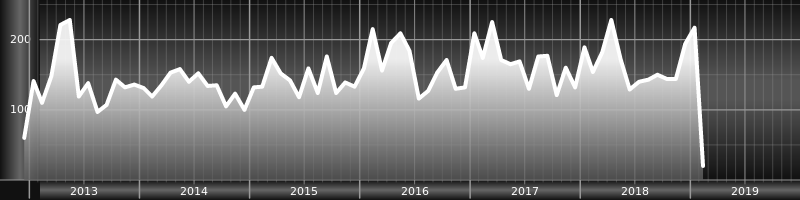
\includegraphics[width=0.75\linewidth]{images/CTAN}}{%
	Caption at top right beside the float and object position left and
the option \texttt{wide}.}{fig:70}
\end{lstlisting}

\hvFloat[%
	wide,nonFloat,
	capPos=right,%
	capVPos=top,%
	objectPos=left,%
]{figure}{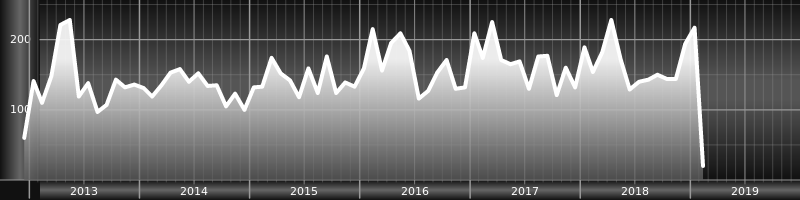
\includegraphics[width=0.75\linewidth]{images/CTAN}}{%
	Caption at top right beside the float and object position left and
the option \texttt{wide}.}{fig:70}

%\blindtext


The code for figure \ref{fig:80}:
\begin{lstlisting}
\hvFloat[wide,nonFloat,
	capPos=left,
	capVPos=top,
	objectPos=right,
  ]{figure}{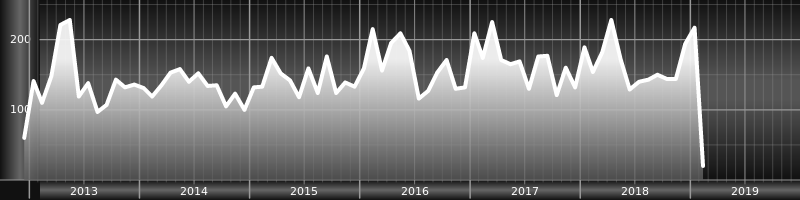
\includegraphics[width=0.75\linewidth]{images/CTAN}}%
  {Caption at top left beside the object and object position left and
   the option \texttt{wide}.}{fig:80}
\end{lstlisting}


\hvFloat[wide,nonFloat,
	capPos=left,%
	capVPos=top,%
]{figure}{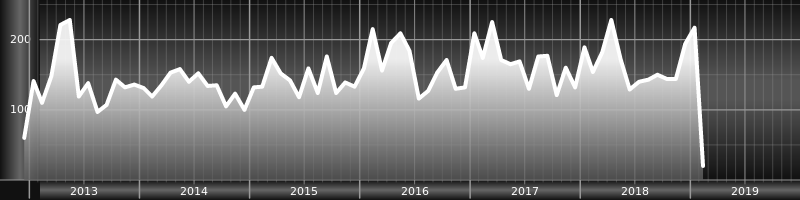
\includegraphics[width=0.75\linewidth]{images/CTAN}}%
  {Caption at top left beside the object and object position left and
   the option \texttt{wide}.}{fig:80}


For a twosided document it will place the object always in the margin.

\blindtext

\begin{lstlisting}
\hvFloat[wide,nonFloat,
	capPos=inner,
	capVPos=top,
]{figure}{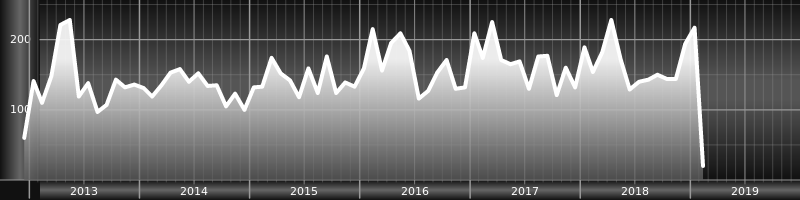
\includegraphics[width=0.75\linewidth]{images/CTAN}}{%
Caption at top and inner beside the float and object position right and
the option \texttt{wide}.}{fig:81}
\end{lstlisting}

\hvFloat[wide,nonFloat,
	capPos=inner,
	capVPos=top,
]{figure}{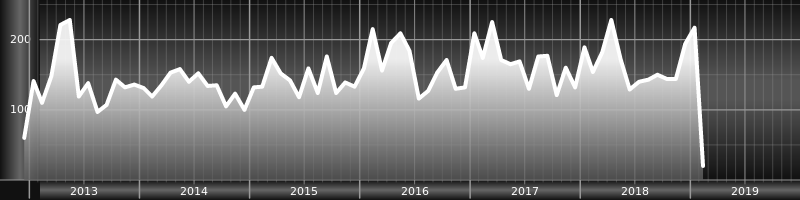
\includegraphics[width=0.75\linewidth]{images/CTAN}}{%
Caption at top and inner beside the float and object position right and
the option \texttt{wide}.}{fig:81}

Now we set the same image with the same setting on the next page. The caption will
change its side due to the setting \Lkeyset{capPos=outer}.

\blindtext



\begin{lstlisting}
\hvFloat[wide,nonFloat,
	capPos=inner,
	capVPos=top,
]{figure}{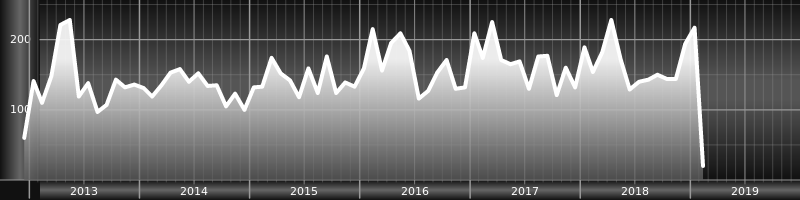
\includegraphics[width=0.75\linewidth]{images/CTAN}}{%
Caption at top inner beside the float and object position right and
the option \texttt{wide}.}{fig:811}
\end{lstlisting}


\hvFloat[wide,nonFloat,
	capPos=inner,
	capVPos=top,
]{figure}{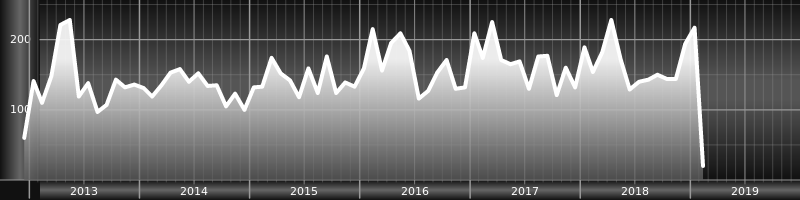
\includegraphics[width=0.75\linewidth]{images/CTAN}}{%
Caption at top inner beside the float and object position right and
the option \texttt{wide}.}{fig:811}

The caption can be typeset completely into the margin with:

\begin{lstlisting}
\captionsetup{justification=RaggedRight}
\hvFloat[wide,nonFloat,
	capPos=outer,
	capVPos=top,
        floatCapSep=\marginparsep,
]{figure}{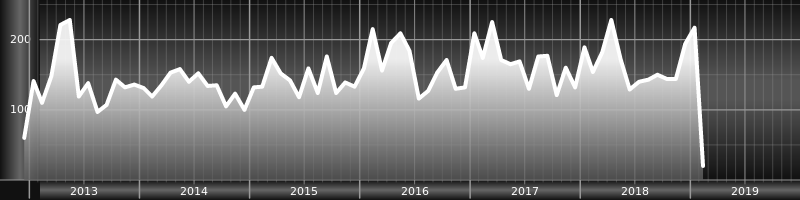
\includegraphics[width=\linewidth]{images/CTAN}}{%
Caption at top inner beside the float and object position right and
the option \texttt{wide}.}{fig:812}
\end{lstlisting}

%\Float[capPos=outer]

\begingroup
\captionsetup{justification=RaggedRight}
\hvFloat[wide,nonFloat,
	capPos=outer,
	capVPos=top,
        floatCapSep=\marginparsep,
]{figure}{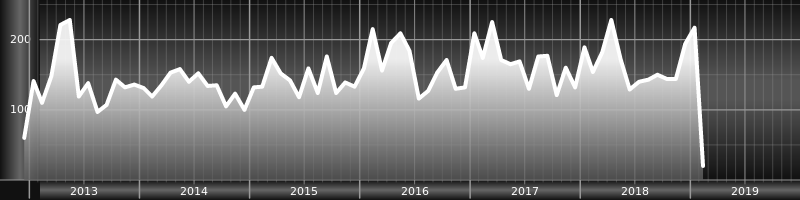
\includegraphics[width=\linewidth]{images/CTAN}}{%
Caption at top inner beside the float and object position right and
the option \texttt{wide}.}{fig:812}
\endgroup

\blindtext
\blindtext

\hvFloat[wide,nonFloat,
	capPos=outer,
	capVPos=top,
        floatCapSep=\marginparsep,
]{figure}{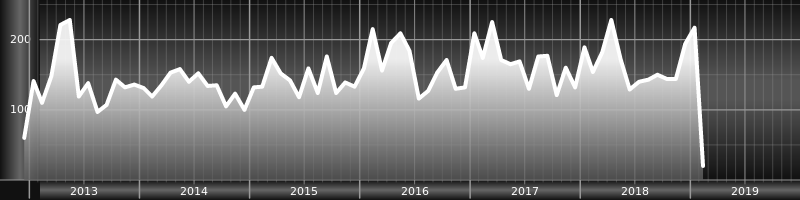
\includegraphics[width=\linewidth]{images/CTAN}}{%
Caption at top inner beside the float and object position right and
the option \texttt{wide}.}{fig:813}





\Blindtext

\end{document} 

